\documentclass[11pt]{article}
\usepackage[margin=1in]{geometry}
\usepackage{amsmath,amssymb,amsthm}
\usepackage{hyperref}
\usepackage{tikz}
\usetikzlibrary{positioning,arrows.meta}
\usepackage{booktabs}
\hypersetup{colorlinks=true,linkcolor=blue,urlcolor=blue}
\newtheorem{definition}{Definition}
\newtheorem{fact}{Fact}
\theoremstyle{definition}\newtheorem{example}{Example}\newtheorem{exercise}{Exercise}
\theoremstyle{remark}\newtheorem*{remark}{Remark}
\newcommand{\op}{\diamond}
\newcommand{\Z}{\mathbb{Z}}
\newcommand{\F}{\mathbb{F}}
\newcommand{\End}{\mathrm{End}}

\title{Everything you need to read the note\\``No constant-coefficient abelian extension of the $\Z/3$ shift refutes $1518\Rightarrow 47,614,817,3862$''}
\author{A backwards tutorial, written for a first-year student}
\date{4 September 2026}

\begin{document}
\maketitle

\section*{How to read this}

The companion note proves one theorem. This document explains every idea the theorem stands on, starting from the theorem and walking \emph{backwards} to things you already know. The picture below is the map: an arrow $A \to B$ means ``you need $A$ to understand $B$''. We will visit the boxes from the bottom up, so that by Section~\ref{sec:theorem} the theorem reads as a plain sentence.

\begin{center}
\resizebox{\textwidth}{!}{%
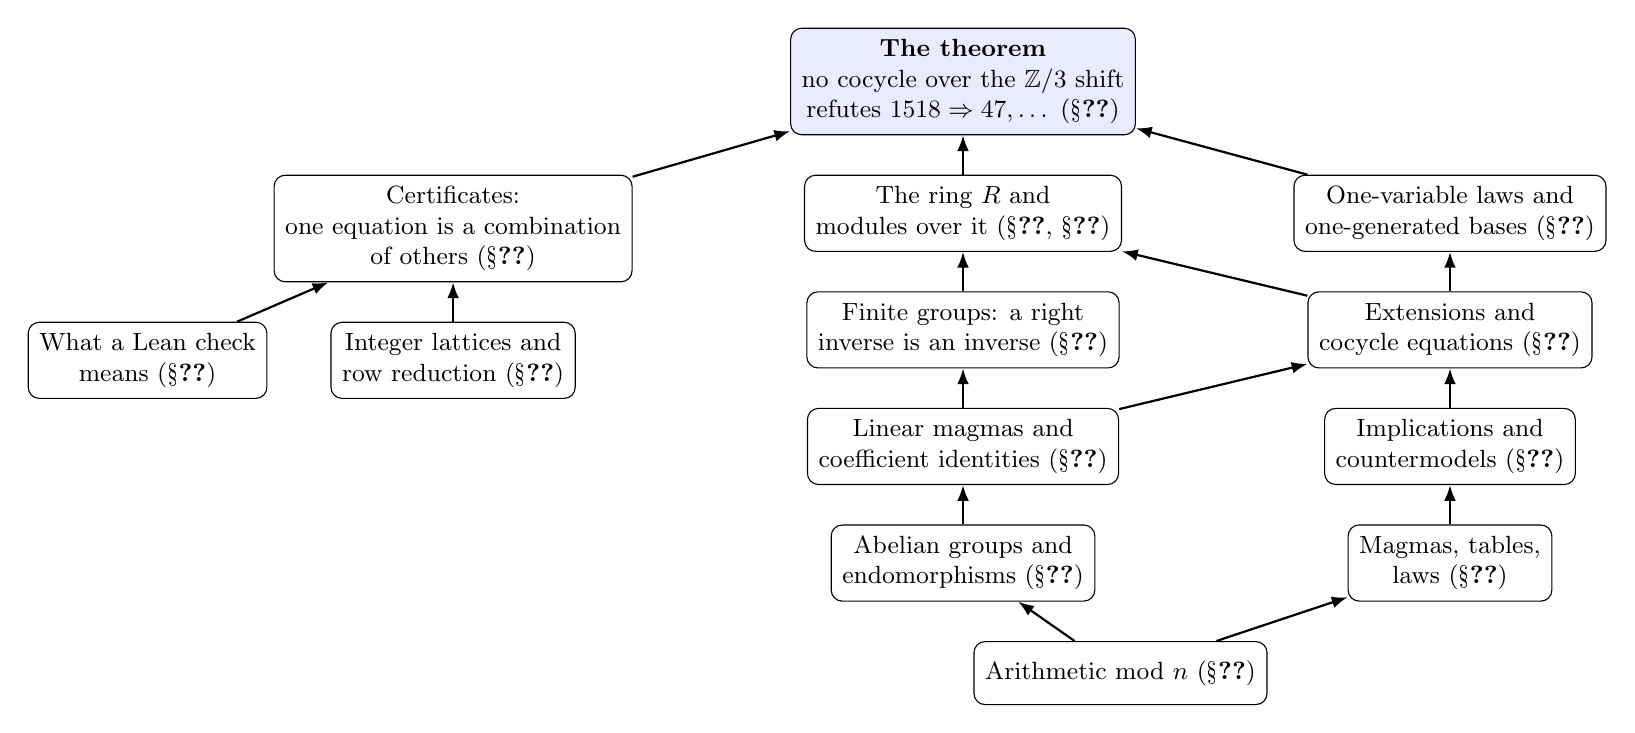
\begin{tikzpicture}[
  node distance=5mm and 6mm,
  box/.style={draw, rounded corners, align=center, font=\small, inner sep=4pt, minimum height=8mm},
  arr/.style={-{Latex[length=2mm]}, thick}]
\node[box, fill=blue!8] (thm) {\textbf{The theorem}\\ no cocycle over the $\Z/3$ shift\\ refutes $1518\Rightarrow 47,\dots$ (§\ref{sec:theorem})};
\node[box, below left=of thm, xshift=-14mm] (cert) {Certificates:\\ one equation is a combination\\ of others (§\ref{sec:linalg})};
\node[box, below=of thm] (ring) {The ring $R$ and\\ modules over it (§\ref{sec:finite}, §\ref{sec:linalg})};
\node[box, below right=of thm, xshift=14mm] (reduce) {One-variable laws and\\ one-generated bases (§\ref{sec:onevar})};
\node[box, below=of cert] (lattice) {Integer lattices and\\ row reduction (§\ref{sec:lattice})};
\node[box, below=of ring] (finite) {Finite groups: a right\\ inverse is an inverse (§\ref{sec:finite})};
\node[box, below=of reduce] (cocycle) {Extensions and\\ cocycle equations (§\ref{sec:ext})};
\node[box, below=of finite] (linear) {Linear magmas and\\ coefficient identities (§\ref{sec:linear})};
\node[box, below=of cocycle] (refute) {Implications and\\ countermodels (§\ref{sec:impl})};
\node[box, below=of linear] (groups) {Abelian groups and\\ endomorphisms (§\ref{sec:groups})};
\node[box, below=of refute] (magma) {Magmas, tables,\\ laws (§\ref{sec:magma})};
\node[box, below=of groups, xshift=20mm] (modn) {Arithmetic mod $n$ (§\ref{sec:modn})};
\node[box, left=of lattice, xshift=-2mm] (lean) {What a Lean check\\ means (§\ref{sec:lean})};
\draw[arr] (cert) -- (thm); \draw[arr] (ring) -- (thm); \draw[arr] (reduce) -- (thm);
\draw[arr] (lattice) -- (cert); \draw[arr] (finite) -- (ring); \draw[arr] (cocycle) -- (reduce); \draw[arr] (cocycle) -- (ring);
\draw[arr] (linear) -- (finite); \draw[arr] (linear) -- (cocycle); \draw[arr] (refute) -- (cocycle);
\draw[arr] (groups) -- (linear); \draw[arr] (magma) -- (refute); \draw[arr] (modn) -- (groups); \draw[arr] (modn) -- (magma);
\draw[arr] (lean) -- (cert);
\end{tikzpicture}}
\end{center}

Nothing here requires more than high-school algebra and a willingness to compute small examples by hand. Every example uses the actual objects of the theorem, so the computations you do here are the computations the proof does.

\section{Arithmetic mod $n$}\label{sec:modn}

$\Z/n$ is the set $\{0,1,\dots,n-1\}$ with addition and multiplication ``wrapped around'': compute as usual, then take the remainder on division by $n$. In $\Z/3$: $2+2=1$, $2\cdot 2=1$. In $\Z/2$: $1+1=0$. We write $x+1$ for the successor in $\Z/3$, so $2+1=0$.

We will use $\Z/3$ as the set on which our main magma lives, $\Z/2$ and $\Z/p$ as ``fibres'', and $\F_p$ as another name for $\Z/p$ when $p$ is prime (then every nonzero element has a multiplicative inverse, which makes $\F_p$ a \emph{field}).

\section{Magmas, tables and laws}\label{sec:magma}

\begin{definition}
A \emph{magma} is a set $G$ with a binary operation $\op\colon G\times G\to G$. No further rule is assumed: not associativity, not commutativity, nothing.
\end{definition}

A finite magma is the same thing as a multiplication table. Our main example:

\begin{example}[the $\Z/3$ shift]\label{ex:shift}
$G=\Z/3$ with $x\op y = y+1$. Its table (row $x$, column $y$):
\[
\begin{array}{c|ccc}
\op & 0 & 1 & 2\\ \hline
0 & 1 & 2 & 0\\
1 & 1 & 2 & 0\\
2 & 1 & 2 & 0
\end{array}
\]
The left argument is ignored; the right argument is shifted by one.
\end{example}

A \emph{law} (or \emph{equation}) is an identity between two expressions built from variables and $\op$, required to hold for \emph{all} values of the variables. The Equational Theories Project (ETP) numbered the 4694 laws with at most four $\op$ symbols. The ones we need:
\begin{align*}
1518:&\quad x = (y \op y) \op (x \op (y \op x)) & 47:&\quad x = x \op (x \op (x \op x))\\
614:&\quad x = x \op (x \op ((x \op x) \op x)) & 817:&\quad x = x \op ((x \op x) \op (x \op x))\\
3862:&\quad x \op x = (x \op (x \op x)) \op x
\end{align*}
Note that 1518 has two variables and the other four have one.

To \emph{check} a law on a finite magma, substitute every possible assignment of values to the variables and evaluate both sides. For 1518 on a 3-element magma that is $3^2=9$ assignments; for 47 it is 3.

\begin{example}
1518 holds on the shift. Take any $x,y\in\Z/3$. Then $y\op y = y+1$, $y\op x = x+1$, $x\op(y\op x)=(x+1)+1=x+2$, and finally $(y+1)\op(x+2) = x+3 = x$. \checkmark\ Law 47 also holds: $x\op x = x+1$, $x\op(x+1)=x+2$, $x\op(x+2)=x+3=x$. \checkmark
\end{example}

\begin{exercise}
Check 3862 on the shift. (Both sides come out $x+1$.)
\end{exercise}

\section{Implications and countermodels}\label{sec:impl}

``Law $E$ implies law $E'$'', written $E\Rightarrow E'$, means: \emph{every} magma satisfying $E$ also satisfies $E'$. To \emph{refute} an implication you need one magma that satisfies $E$ and violates $E'$; such a magma is a \emph{countermodel}. One finite table suffices, because ``every magma'' includes it.

Two flavours matter. The ETP settled $E\Rightarrow E'$ for all $4694^2$ pairs among \emph{all} magmas, and separately among \emph{finite} magmas. For our five laws the finite answer is: 1518 does not imply any of 47, 614, 817, 3862 among finite magmas. The smallest finite countermodel to $1518\Rightarrow47$ has 15 elements (Brox and Le Floch, 2025), and the ETP's 15-element table \texttt{Refutation939} refutes all four at once. We will meet that table again in Section~\ref{sec:theorem}.

The theorem in the companion note is \emph{not} about whether the implication is true (it is false). It is about whether a particular \emph{method} of building countermodels can ever succeed. That method is the subject of Sections~\ref{sec:groups}--\ref{sec:ext}.

\section{Abelian groups and endomorphisms}\label{sec:groups}

\begin{definition}
An \emph{abelian group} is a set $M$ with an addition $+$ that is associative and commutative, has a zero, and where every element $s$ has a negative $-s$. Examples: $\Z/n$; pairs $(u,v)$ with $u,v\in\Z/p$ added componentwise, written $(\Z/p)^2$.
\end{definition}

\begin{definition}
An \emph{endomorphism} of $M$ is a map $\varphi\colon M\to M$ that respects addition: $\varphi(s+t)=\varphi(s)+\varphi(t)$. The set of all of them is $\End(M)$. Endomorphisms can be added pointwise and composed; composition plays the role of multiplication, and we write $\varphi\psi$ for ``first $\psi$, then $\varphi$''.
\end{definition}

\begin{example}
Every endomorphism of $\Z/p$ is ``multiply by a fixed number $c$'': $\varphi(s)=cs$. So $\End(\Z/p)$ is just $\Z/p$ itself, with ordinary multiplication. Every endomorphism of $(\Z/p)^2$ is a $2\times 2$ matrix with entries in $\Z/p$, acting on column vectors; here two endomorphisms need not commute.
\end{example}

A polynomial identity like $\beta^5+\beta^3-\beta^2-1=0$ for $\beta\in\End(M)$ means: for every $s\in M$, applying $\beta$ five times, plus three times, minus twice, minus once, gives $0$. When $M=\Z/p$ and $\beta$ is ``multiply by $r$'' this is the ordinary statement $r^5+r^3-r^2-1\equiv 0 \pmod p$.

\section{Linear magmas and coefficient identities}\label{sec:linear}

Given $M$ and $\alpha,\beta\in\End(M)$, define an operation on $M$ by
\[
s \op t = \alpha s + \beta t .
\]
This is a \emph{linear magma}. Which laws does it satisfy? Expand both sides of the law; because $\alpha,\beta$ respect addition, each side becomes a sum of the variables with endomorphism coefficients, and the law holds if and only if the coefficient of each variable agrees on both sides.

\begin{example}[1518 on a linear magma]\label{ex:lin1518}
With $s\op t=\alpha s+\beta t$ and variables $x,y$:
\begin{align*}
y\op y &= (\alpha+\beta)\,y,\\
y\op x &= \alpha y+\beta x,\\
x\op(y\op x) &= \alpha x + \beta(\alpha y + \beta x) = (\alpha+\beta^2)\,x + \beta\alpha\, y,\\
(y\op y)\op(x\op(y\op x)) &= \alpha(\alpha+\beta)y + \beta\bigl((\alpha+\beta^2)x+\beta\alpha y\bigr)
 = (\beta\alpha+\beta^3)\,x + (\alpha^2+\alpha\beta+\beta^2\alpha)\,y .
\end{align*}
The law says this equals $x$, so the linear magma satisfies 1518 exactly when
\[
\beta\alpha+\beta^3 = 1 \qquad\text{and}\qquad \alpha^2+\alpha\beta+\beta^2\alpha = 0 .
\]
\end{example}

\begin{example}[the smallest fibre]\label{ex:z2}
$M=\Z/2$, $\alpha=0$, $\beta=1$. Then $\beta\alpha+\beta^3 = 0+1 = 1$ \checkmark\ and $\alpha^2+\alpha\beta+\beta^2\alpha = 0$ \checkmark. So $s\op t = t$ on $\Z/2$ is a 1518-magma. It is also a 47-magma: $x\op(x\op(x\op x)) = x$ because the operation always returns its right argument. Same for 614, 817, 3862.
\end{example}

This example is not an accident. The companion note checks that \emph{every} linear 1518-magma with finite $M$ satisfies all four targets, so a linear magma alone can never be a countermodel. That is why one needs the extension construction next.

\section{Extensions and cocycle equations}\label{sec:ext}

The idea, from the ETP's ``magma cohomology'' chapter: glue a base magma $G$ and a linear magma $M$ into a bigger magma on the set of pairs $G\times M$, and add a correction term.

\begin{definition}
Let $G$ be a magma, $M$ an abelian group, $\alpha,\beta\in\End(M)$, and $f\colon G\times G\to M$ any function. The \emph{extension} is the magma on $G\times M$ with
\begin{equation}\label{eq:ext}
(x,s)\op(y,t) = \bigl(x\op y,\ \alpha s+\beta t+f(x,y)\bigr).
\end{equation}
The first coordinate is computed in $G$ (the \emph{base}); the second in $M$ (the \emph{fibre}) using the linear magma plus the correction $f$, which depends only on the base coordinates. The coefficients $\alpha,\beta$ are the same for all $x,y$: \emph{constant coefficients}.
\end{definition}

If $f=0$ this is just the direct product: two magmas running side by side. The function $f$ is what makes the construction interesting.

\paragraph{When does the extension satisfy a law?} Suppose $G$ and the linear magma both satisfy $E$. Evaluate any word in the extension: the base coordinate is the word evaluated in $G$; the fibre coordinate is the word evaluated in the linear magma \emph{plus} a sum of $f$-values with endomorphism coefficients, one $f$-value for each $\op$ in the word. Because $G$ satisfies $E$, the base coordinates of both sides agree. Because the linear magma satisfies $E$, the $s,t$ parts agree. What remains is a condition on $f$ alone, and it is \emph{linear} in $f$. A function $f$ satisfying it is called an \emph{$E$-cocycle}.

\begin{example}[the 1518 cocycle equation over the shift]\label{ex:cocycle}
Base: the $\Z/3$ shift. Fibre: any $(M,\alpha,\beta)$ satisfying 1518. Compute the right side of 1518 at $(x,s),(y,t)$, keeping only the $f$-terms (the base and the $s,t$ parts we already know agree):
\begin{align*}
(y,t)\op(y,t) &\rightsquigarrow \bigl(y+1,\ f(y,y)+\cdots\bigr),\\
(y,t)\op(x,s) &\rightsquigarrow \bigl(x+1,\ f(y,x)+\cdots\bigr),\\
(x,s)\op\bigl((y,t)\op(x,s)\bigr) &\rightsquigarrow \bigl(x+2,\ \beta f(y,x)+f(x,x+1)+\cdots\bigr),\\
\bigl((y,t)\op(y,t)\bigr)\op\bigl(\cdots\bigr) &\rightsquigarrow \bigl(x,\ \alpha f(y,y)+\beta^2 f(y,x)+\beta f(x,x+1)+f(y+1,x+2)+\cdots\bigr).
\end{align*}
Each time we multiply, the left fibre gets $\alpha$ in front, the right fibre gets $\beta$, and a new $f$-value is added, indexed by the two \emph{base} coordinates being multiplied. The left side of the law is $(x,s)$, whose fibre has no $f$-term. So $f$ is a 1518-cocycle exactly when, for all $x,y\in\Z/3$,
\begin{equation}\label{eq:c1518}
\alpha\, f(y,y) + \beta^2 f(y,x) + \beta\, f(x,x+1) + f(y+1,x+2) = 0 .
\end{equation}
Nine equations (one per pair $(x,y)$) in nine unknowns $f(0,0),\dots,f(2,2)$.
\end{example}

\begin{example}[the 47 cocycle equation]
Same procedure with $x\op(x\op(x\op x))$: $x\op x\rightsquigarrow f(x,x)$; $x\op(x\op x)\rightsquigarrow \beta f(x,x)+f(x,x+1)$; $x\op(\cdots)\rightsquigarrow \beta^2 f(x,x)+\beta f(x,x+1)+f(x,x+2)$. So $f$ is a 47-cocycle when
\begin{equation}\label{eq:c47}
\beta^2 f(x,x)+\beta f(x,x+1)+f(x,x+2)=0 \qquad (x\in\Z/3).
\end{equation}
\end{example}

\begin{example}[everything by hand, with the $\Z/2$ fibre]\label{ex:z2cocycles}
Take the fibre of Example~\ref{ex:z2}: $M=\Z/2$, $\alpha=0$, $\beta=1$. Equation~\eqref{eq:c1518} becomes, mod 2,
\[
f(y,x)+f(x,x+1)+f(y+1,x+2)=0 .
\]
Nine equations, nine unknown bits. Solving them (try it: start from $x=y$) gives exactly four solutions. Writing $f$ as a $3\times3$ array with row $x$ and column $y$:
\[
\begin{pmatrix}0&0&0\\0&0&0\\0&0&0\end{pmatrix},\quad
\begin{pmatrix}0&1&1\\0&1&1\\0&1&1\end{pmatrix},\quad
\begin{pmatrix}1&0&1\\1&0&1\\1&0&1\end{pmatrix},\quad
\begin{pmatrix}1&1&0\\1&1&0\\1&1&0\end{pmatrix}.
\]
Each depends on $y$ only, and each has the form $f(x,y)=g(y)+g(y+1)$ for some $g\colon\Z/3\to\Z/2$. Now check the 47 equation~\eqref{eq:c47}, which mod 2 reads $f(x,x)+f(x,x+1)+f(x,x+2)=0$: for every one of the four arrays the row sum is $0$. \checkmark\ So none of the four extensions is a countermodel to $1518\Rightarrow 47$. The theorem says this keeps happening for \emph{every} finite fibre, not just $\Z/2$.
\end{example}

\begin{remark}
Functions of the form $f(x,y)=g(x\op y)-\alpha g(x)-\beta g(y)$ are called \emph{coboundaries}. They are always cocycles, and an extension by a coboundary is just the direct product in disguise (relabel $(x,s)\mapsto (x,s+g(x))$). In Example~\ref{ex:z2cocycles} all four cocycles are coboundaries, so those four extensions are all secretly the direct product. Cohomology is the study of cocycles \emph{modulo} coboundaries: the quotient $H^{2}=Z^{2}/B^{2}$ measures how many genuinely new extensions there are. The companion note's Section~4 shows that for the $\Z/3$ shift and \emph{every} finite 1518-fibre, $H^{2}=0$: what happened in the toy example always happens. That is the real reason the four target laws cannot be broken, since a direct product satisfies every law its two factors satisfy. By contrast, for the 879 base of the next paragraph $H^{2}$ has dimension 2, which is exactly the room the method needed there.
\end{remark}

\paragraph{How the method refutes an implication.} If $f$ is an $E$-cocycle but \emph{not} an $E'$-cocycle, then the extension satisfies $E$ and violates $E'$: a countermodel. This is how the ETP refuted $879\Rightarrow4065$ in November 2024: base $\Z/6$ with $x\op y = 3x+y+1$, fibre $\Z/2$, $\alpha=\beta=1$; there the 879 cocycle equations have $2^7$ solutions and $64$ of them fail the 4065 equation. Twelve elements, the smallest possible. The same people tried the same thing for 1518 and found nothing. The theorem explains why.

\section{One-variable laws and one-generated bases}\label{sec:onevar}

The four target laws use only $x$. Evaluating such a law at an element $(x,s)$ of the extension only ever multiplies elements that came from $(x,s)$ itself. So all the base coordinates that appear lie in the \emph{submagma generated by $x$}: the smallest subset of $G$ containing $x$ and closed under $\op$, written $\langle x\rangle$.

Consequence (Tao, November 2024): if some extension of $G$ violates a one-variable law at $(x,s)$, then the extension of the smaller base $\langle x\rangle$, with the same fibre and the restriction of $f$, also violates it. So to decide whether the method can ever produce a countermodel, it is enough to look at bases generated by a single element, the \emph{one-generated} 1518-magmas.

\begin{example}
In the shift, $\langle 0\rangle = \{0, 0\op0=1, 1\op 1 = 2\} = \Z/3$: the shift is one-generated. In a magma where $x\op x = x$ for all $x$ (an \emph{idempotent} magma), $\langle x\rangle=\{x\}$: a one-element base, on which nothing interesting can happen.
\end{example}

A computer census (the program Mace4, which lists all finite magmas satisfying a given law) shows: among 1518-magmas with at most 8 elements, the only one-generated ones are the trivial one-element magma and the $\Z/3$ shift (for sizes 2 to 8 this is also a Lean theorem, proved through a SAT solver whose proof Lean checks). That is why the theorem is about the shift.

\section{Finite groups: a right inverse is an inverse}\label{sec:finite}

Here is the one step where finiteness is used, and it is elementary.

\begin{fact}\label{fact:bij}
Let $M$ be a finite set and $\beta\colon M\to M$ a map with a right inverse, i.e.\ some $\gamma$ with $\beta(\gamma(s))=s$ for all $s$. Then $\beta$ is a bijection and $\gamma$ is its inverse.
\end{fact}
\begin{proof}
$\beta\circ\gamma=\mathrm{id}$ means every $s$ is hit by $\beta$: $\beta$ is surjective. A surjective map from a finite set to itself is injective (pigeonhole), hence bijective, and then $\gamma=\beta^{-1}$.
\end{proof}

Apply this to the first identity of Example~\ref{ex:lin1518}: $\beta\alpha+\beta^3=1$ says $\beta(\alpha+\beta^2)=1$, so $\alpha+\beta^2$ is a right inverse of $\beta$. If $M$ is finite, $\beta$ is invertible and
\[
\alpha = \beta^{-1}-\beta^2 .
\]
Two things follow. First, $\alpha$ is built from $\beta$ alone, so $\alpha$ and $\beta$ commute (a matrix commutes with polynomials in itself and its inverse). Second, substitute into the second identity, using commutativity:
\begin{align*}
\alpha^2+\alpha\beta+\beta^2\alpha &= \alpha^2+\alpha(\beta+\beta^2)
= (\beta^{-1}-\beta^2)^2 + (\beta^{-1}-\beta^2)(\beta+\beta^2)\\
&= (\beta^{-2}-2\beta+\beta^4) + (1+\beta-\beta^3-\beta^4)
= \beta^{-2} - \beta - \beta^{3} + 1 = 0,
\end{align*}
and multiplying by $\beta^2$:
\[
\beta^5+\beta^3-\beta^2-1 = 0, \qquad\text{i.e.}\qquad (\beta^2+1)(\beta^3-1)=0 .
\]
Conversely, if $\beta$ satisfies this polynomial and $\alpha:=\beta^{-1}-\beta^2$, both identities hold. So:

\begin{fact}\label{fact:ring}
For finite $M$, the linear magma $\alpha s+\beta t$ satisfies 1518 if and only if $\beta$ satisfies $\beta^5+\beta^3-\beta^2-1=0$ and $\alpha=\beta^{-1}-\beta^2$.
\end{fact}

\begin{example}
On $\Z/2$: $\beta=1$ gives $1+1-1-1=0$ \checkmark, and $\alpha=1-1=0$. That is Example~\ref{ex:z2}. On $\Z/5$: $r^5+r^3-r^2-1\equiv0$ has the roots $r=1,2,3$; for $r=2$, $\alpha = 2^{-1}-4 = 3-4 = -1 = 4$, so $s\op t = 4s+2t$ is a 1518-magma on $\Z/5$.
\end{example}

\paragraph{The ring $R$.} Fact~\ref{fact:ring} says every finite fibre is governed by one symbol $b$ obeying one polynomial rule. Formalise that as the ring
\[
R = \Z[b]\big/(b^5+b^3-b^2-1):
\]
polynomials in $b$ with integer coefficients, where $b^5$ may be replaced by $-b^3+b^2+1$ whenever it appears. Every element of $R$ can be written uniquely as $c_0+c_1b+c_2b^2+c_3b^3+c_4b^4$ with integers $c_i$: five coordinates. In $R$, $b$ is invertible: $b\cdot(b^4+b^2-b)=b^5+b^3-b^2=1$. Set $a:=b^{-1}-b^2 = b^4-b$.

Saying ``$M$ is an $R$-module'' just means: $M$ is an abelian group on which $b$ acts as an endomorphism $\beta$ satisfying the polynomial rule; then $a$ acts as $\alpha$. Fact~\ref{fact:ring} in these words: \emph{the finite 1518 fibres are exactly the finite $R$-modules}. This turns infinitely many cases (all $M$, all $\alpha,\beta$) into one algebraic object.

\section{Kernels, containment and certificates}\label{sec:linalg}

Write the nine cocycle equations~\eqref{eq:c1518} with $\alpha=a$, $\beta=b$ as a $9\times 9$ matrix $D_{1518}$ with entries in $R$: row $(x,y)$ lists the coefficient of each unknown $f(x',y')$. For a given fibre $M$, the 1518-cocycles are the vectors $f\in M^9$ with $D_{1518}f=0$: the \emph{kernel}. Likewise the three equations~\eqref{eq:c47} give a $3\times9$ matrix $D_{47}$.

The theorem says: $\ker D_{1518}\subseteq\ker D_{47}$ for every finite $R$-module $M$ (and the same for 614, 817, 3862).

\paragraph{Certificates.} Here is a way to prove such a containment that a computer can find and anyone can check. Suppose there is a matrix $C$ with entries in $R$ such that
\[
C\cdot D_{1518} = D_{47}\qquad\text{entrywise in } R.
\]
Then for any $f$ with $D_{1518}f=0$ we get $D_{47}f = C\,D_{1518}f = C\cdot 0 = 0$. Done, for every module at once, because the identity $C D_{1518}=D_{47}$ is a statement about polynomials in $b$ and survives substituting any $\beta$ that obeys the rule. $C$ is the \emph{certificate}.

\begin{example}[a toy certificate over the integers]
Equations $E_1: 2u+v=0$ and $E_2: u-v=0$. The equation $E_3: 3u=0$ is their sum, $E_3=E_1+E_2$, so the certificate is $C=(1\ \ 1)$, and every solution of $E_1,E_2$ satisfies $E_3$.
\end{example}

\begin{example}[the real one]
Writing $r_{xy}$ for row $(x,y)$ of $D_{1518}$, the companion note exhibits
\[
D_{47}(0) = r_{00}+(b-b^2-b^4)\,r_{11}+(-1+b+b^3)\,r_{20},
\]
and similar combinations for the other rows and the other three targets. To check one such identity you multiply polynomials in $b$, replace $b^5$ by $-b^3+b^2+1$, and compare coefficients. It is tedious and completely mechanical, which is exactly what makes it checkable by a machine (Section~\ref{sec:lean}).
\end{example}

\section{Integer lattices: how the certificate was found}\label{sec:lattice}

Finding $C$ means answering: is each row of $D_{47}$ an $R$-combination of the rows of $D_{1518}$? Since every element of $R$ is five integers, an $R$-combination $\sum_j c_j r_j$ with $c_j = \sum_i c_{ji}b^i$ is an \emph{integer} combination of the 45 vectors $b^i r_j$ ($j=1..9$, $i=0..4$), each living in $\Z^{45}$ (nine entries times five coordinates). The set of all integer combinations of a finite list of integer vectors is a \emph{lattice}, and membership in a lattice is decided by integer row reduction: bring the generators to echelon form using only integer operations (subtracting multiples of rows, with Euclid's algorithm on each pivot column), then peel the target vector off pivot by pivot, checking divisibility at each step. If it reduces to zero, the recorded multipliers give $C$; if not, the target is outside the lattice.

For the $\Z/3$ shift the 45 generators span a lattice of rank 35 inside $\Z^{45}$; all fifteen target generators (five per row, three rows, for each of the four targets) reduce to zero. Had one not, the leftover would have produced an explicit finite fibre and cocycle refuting the implication, so the computation could not have ended inconclusively.

\section{What a Lean check means}\label{sec:lean}

Lean is a proof assistant: a program whose small trusted core (the \emph{kernel}) accepts a statement only if it is given a complete proof it can verify step by step. The companion note's file \texttt{L2Cert.lean} contains the matrices $D_{1518}$, $D_{47},\dots$ and the certificates $C$ as literal lists of integers, a definition of multiplication in $R$, and the five statements $C\cdot D_{1518}=D_{E'}$. The tactic \texttt{decide} makes the kernel compute both sides and compare them. The output line \texttt{depends on axioms: [propext]} says the check used only a standard, harmless axiom, and in particular no ``trust me'' escape hatch.

What this does \emph{not} check: that the matrices really are the cocycle conditions of those laws over the shift (Section~\ref{sec:ext}), and that finite fibres are $R$-modules (Section~\ref{sec:finite}). Those are the short arguments you have just read. A full formalisation would encode them too; it has not been done.

\section{The theorem, re-read}\label{sec:theorem}

\begin{quote}
Let $G$ be the $\Z/3$ shift (or the one-element magma), $M$ a finite abelian group, $\alpha,\beta\in\End(M)$ with $\alpha s+\beta t$ a 1518-magma. Then every 1518-cocycle $f\colon G\times G\to M$ is a 47-, 614-, 817- and 3862-cocycle. Hence no extension~\eqref{eq:ext} of $G$ refutes $1518\Rightarrow E'$ for these four $E'$.
\end{quote}

In the words of this tutorial: whatever finite fibre you choose (Section~\ref{sec:finite} says it is an $R$-module), and whatever correction $f$ you choose that keeps 1518 true (Section~\ref{sec:ext}: a solution of the nine equations), the four target laws stay true too (Section~\ref{sec:linalg}: because their equations are combinations of the nine). The stronger form proved in the note says why: every such $f$ is a coboundary, so the extension is the direct product with its elements renamed, and a direct product breaks no law that both factors obey. The extension construction with constant coefficients over this base is therefore useless not just for these four implications but for every implication from 1518 whose target holds in the shift and in all finite linear 1518-magmas.

\paragraph{The corollary, and then the theorem.} Since (Section~\ref{sec:onevar}) one may shrink the base to $\langle x\rangle$, and (census) the only one-generated 1518-magmas with at most 8 elements are trivial or the shift, any constant-coefficient extension that \emph{does} refute one of these implications must have a base containing a one-generated submagma of at least 9 elements. Tao conjectured in 2024 that no such base exists. This is now a theorem, and it needs neither the census nor finiteness: in any magma satisfying 1518 and 3862, writing $A=x\op x$ and $B=A\op A$, every product of two elements of $\{x,A,B\}$ equals $S$ of the right factor, and $B\op B=x$. So $\{x,A,B\}$ is closed under $\op$, carries the shift's multiplication table, and has one element or three. Every one-generated magma satisfying 1518 and 3862 is trivial or the $\Z/3$ shift. The nine product identities were found by the prover Vampire from the two laws alone and then written out as Lean proofs (\texttt{research/audit/lean/OneGenerated1518.lean}), where the table and the closure of words check with no axioms at all. Consequence, with the theorem of this tutorial: a constant-coefficient extension of a \emph{finite} 1518-magma violates one of 47, 614, 817, 3862 only if the base already does (the four laws are equivalent in finite 1518-magmas, another Vampire result). The method is useless for these four implications from any finite base.

\paragraph{Where the line is.} The theorem says nothing about extensions whose coefficients $\alpha_{x,y},\beta_{x,y}$ change with the base pair, about extensions of extensions, or about fibres where Fact~\ref{fact:bij} fails. The first of these is not a technicality. The ETP's 15-element countermodel \texttt{Refutation939} is itself an extension of the $\Z/3$ shift by $\Z/5$: it has a quotient isomorphic to the shift, with classes of five elements, and after labelling each class by $\Z/5$ its operation reads $(x,s)\op(y,t)=(y+1,\ \alpha_{x,y}s+\beta_{x,y}t+c_{x,y})$ with $\alpha_{x,y}\in\{1,2,4\}$ and $\beta_{x,y}\in\{1,2,3,4\}$ depending on the pair $(x,y)$. The theorem shows no relabelling can make those coefficients constant. So over this base the picture is complete: constant coefficients give only direct products in disguise; letting the coefficients vary gives the smallest countermodel there is. The theorem is also not a claim of novelty: the search for a prior statement came back empty, which is different from a proof that there is none.

\begin{exercise}
Redo Example~\ref{ex:z2cocycles} for the fibre $\Z/5$ with $\beta=2$, $\alpha=4$ (from the example in Section~\ref{sec:finite}). The nine equations~\eqref{eq:c1518} become $4f(y,y)+4f(y,x)+2f(x,x+1)+f(y+1,x+2)=0 \pmod 5$. There are $25$ solutions. Check that each satisfies~\eqref{eq:c47}: $4f(x,x)+2f(x,x+1)+f(x,x+2)=0 \pmod 5$. (A short program is fine; this is exactly the ``numeric cross-check'' row of the note's verification table.)
\end{exercise}

\end{document}
